
To estimate the effect of photoelectrons on the buildup simulations, a simulation study that includes the common magnets in a cryogenic cell of the LHC is presented here.
Each of these magnets is simulated either with photoemission seeding or with an initial distribution of electrons.
The normally used magnetic fields for a beam with an energy of 6.5~TeV are shown in the following table, its content has been extracted either from MADX files or from the settings of the LHC control system for a standard physics fill in 2016.
Their lengths have been inferred from MADX input files for the LHC.
\begin{center}
    \begin{tabular}{llll}
        \textbf{Magnet} & \textbf{Length} [m]&\textbf{B} & \textbf{B\_skew}\\ \hline
        Drift & 5.79 & - & - \\
        Main Bend & 42.90 & 7.73 T& - \\
        Horizontal corrector magnet & 0.32 & 2.72 T & - \\
        Vertical corrector magnet & 0.32 & - & 2.32 T \\
        Main quadrupole & 3.46 & 174.78 T/m& - \\
        Main sextupole ($+$)& 0.35 & 758.86 T/m$^2$ & - \\
        Main sextupole ($-$) & 0.35 & -1300.9 T/m$^2$ & - \\
        Main octupole & 0.15 & 57817.78 T/m$^3$ & - \\
    \end{tabular}
\end{center}

Figure~\ref{fig:simulation} shows the heat loads per meter for a two trains of 288 bunches, consisting of 4 batches with 72 bunches.
The batches are interleaved with 8 bunches, and the trains with 30 bunches.
The heat load from the second train has been rescaled to 
The bunch intensity was set to 1.1$\cdot10^{11}$ p/b.
The right axes correspond to the heat load scaled to the length each element has in a typical cryogenic cell of the LHC arcs.
\\
So far, only simulations with the conservative estimates for the photoemission parameters have been run.
It is clear that dipoles, quadrupoles and drift spaces are most relevant in terms of total heat load.
Furthermore, the photoemission seeding only has a significant impact on drifts and dipoles.

Figure~\ref{fig:summed_hl} shows the summed up heat loads, with the same SEY for all devices or some selected combinations that cover the range of observed heat loads in the arcs.
Additionally, also the expected contributions from the resistive wall effect and the absorption of synchrotron radiation are shown.


\begin{figure}[tbh]
    \centering
    \begin{minipage}[c]{0.8\textwidth}
        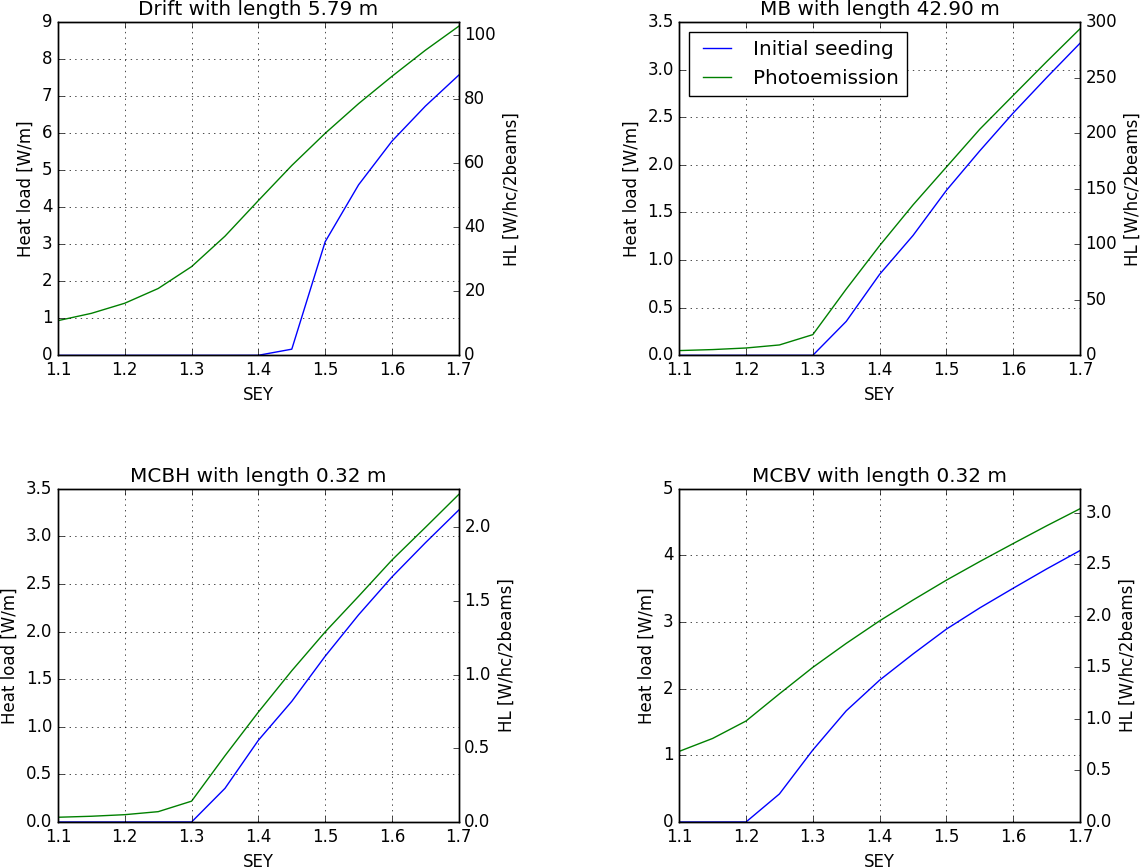
\includegraphics[width=\textwidth]{../plots/study_2.png}
    \end{minipage}

    \vspace{0.5cm}

    \begin{minipage}[c]{0.8\textwidth}
        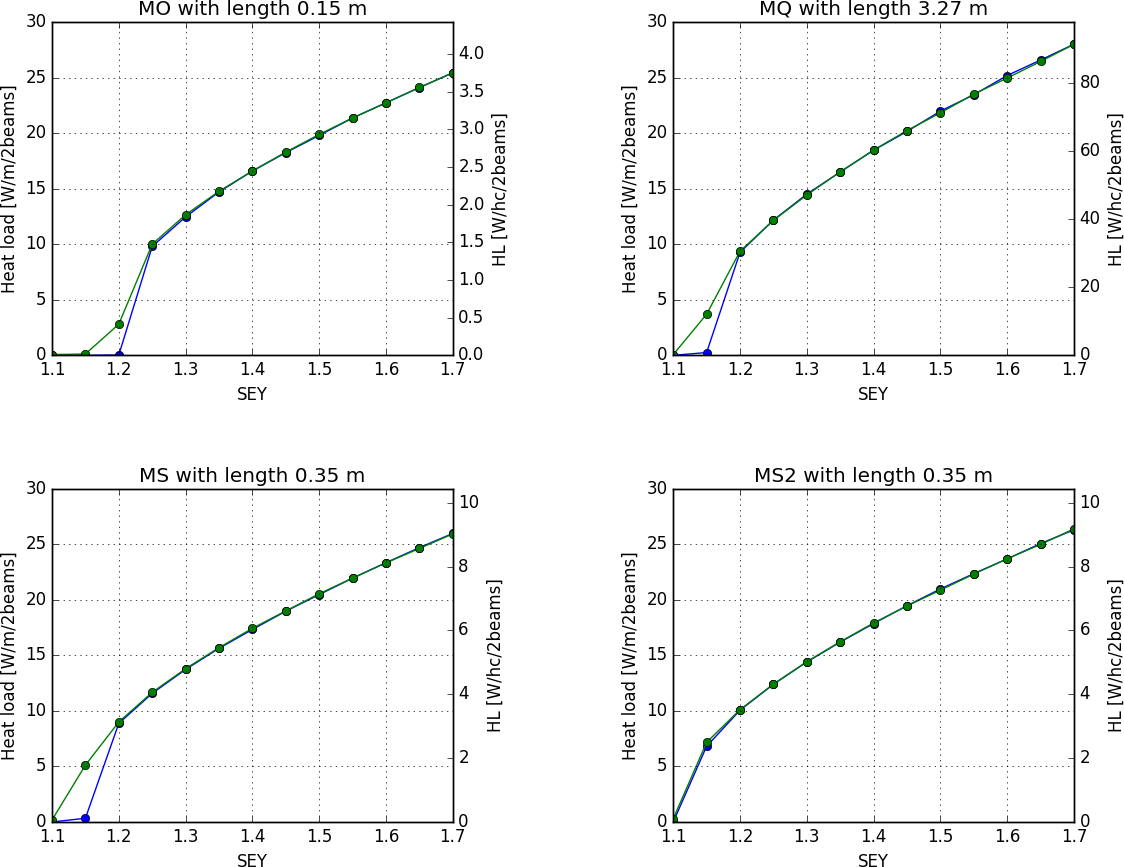
\includegraphics[width=\textwidth]{../plots/study_3.png}
    \end{minipage}
    \caption{These are the resulting heat loads from simulations with "conservative" photoemission parameters derived in Sec.~\ref{sec:best} and magnetic field parameters from Sec.~\ref{sec:simulation}.}
    \label{fig:simulation}
\end{figure}


\begin{figure}[tbh]
    \centering
    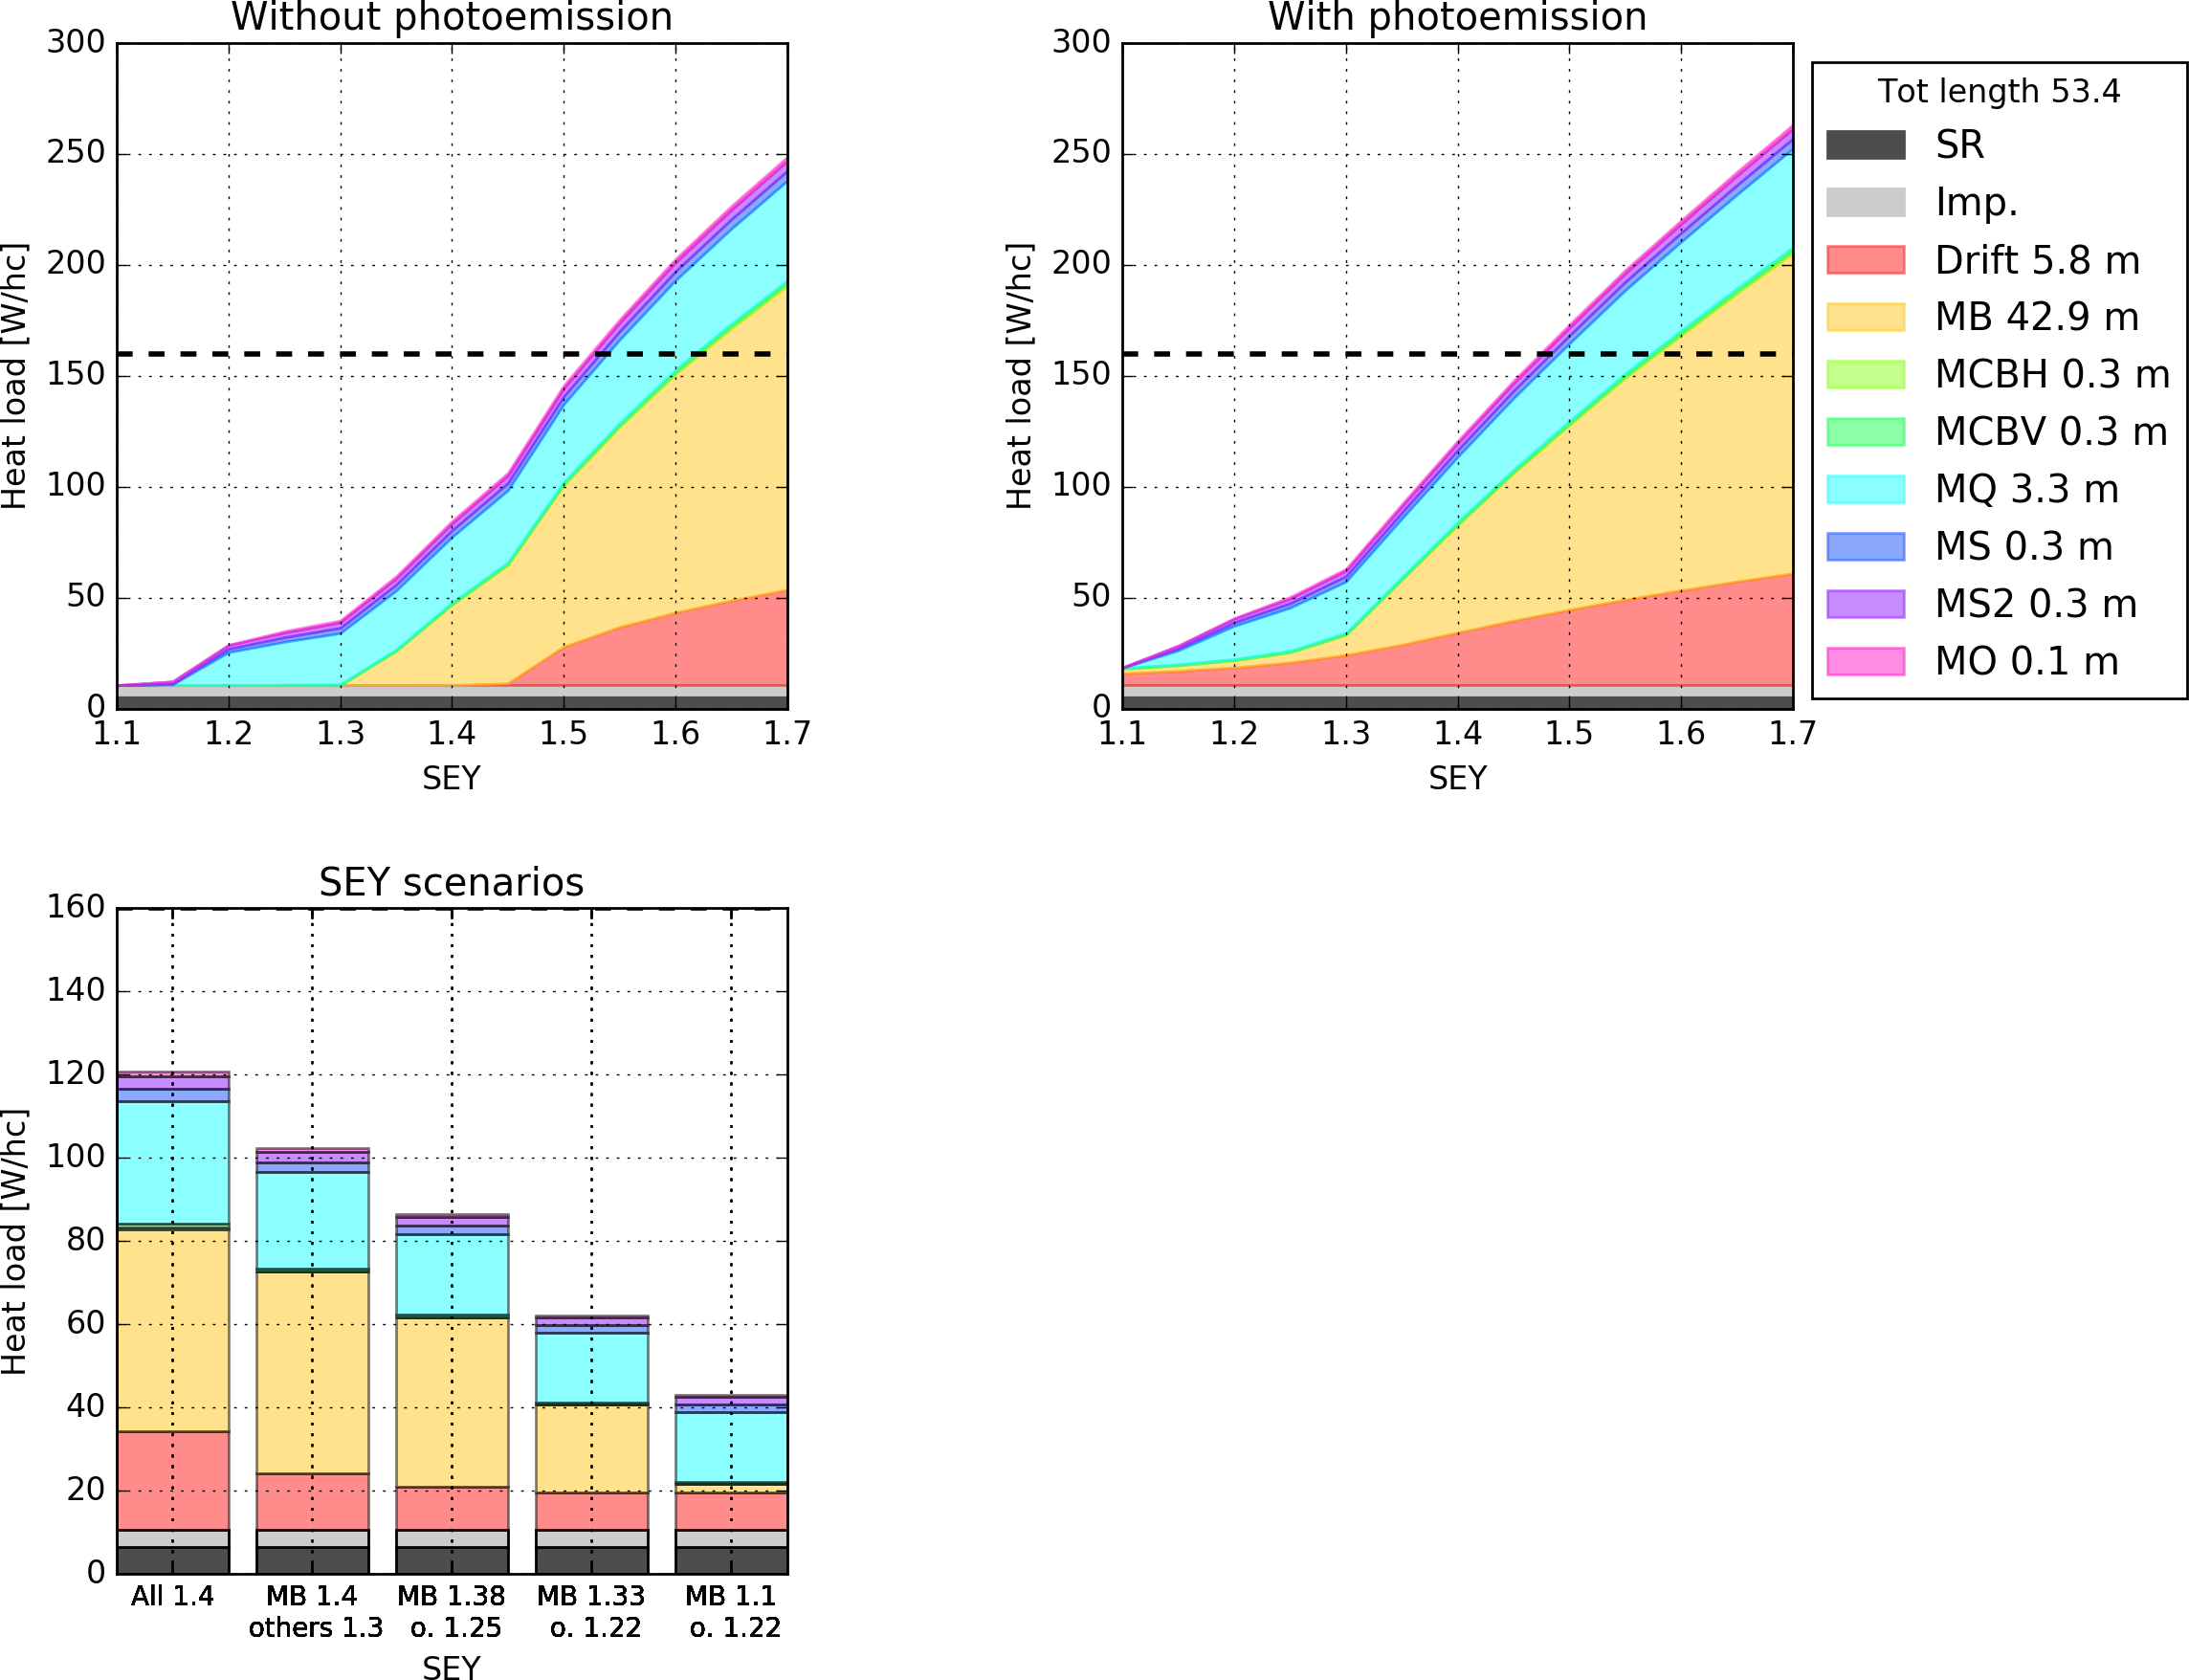
\includegraphics[width=0.8\textwidth]{../plots/summed_hl_1.png}
    \caption{The top two plots add up the heat loads for the same value of the SEY, which gives a rough overview about the relative impact of each element.
    The bottom plot shows the cumulative heat loads for different combinations of SEY values.
    }
    \label{fig:summed_hl}
\end{figure}

